\documentclass{beamer}
\usetheme{metropolis}           
\usepackage[utf8]{inputenc}
\usepackage{graphicx,color}
\usepackage[dvipsnames]{xcolor}
\usepackage{cite} 
\useinnertheme{circles}
\graphicspath{{../figures/}}


\title{Nanoscale hydrodynamics near solids}
\date{June 2019}
\author{Diego Duque Zumajo}
\institute{Departamento Física Fundamental \\Universidad Nacional de Educación a Distancia}

% logo of my university
\titlegraphic{%
\begin{picture}(0,0)
\put(308,-119){\makebox(0,0)[rt]{\includegraphics[width=1.5cm]{logo}}}
\end{picture}}
%\AtBeginSection[]{
%\begin{frame}{Agenda}
%\tableofcontents[currentsection]
%\end{frame}
%\frame{\sectionpage}
%}

\begin{document}
\maketitle

%\begin{frame}
%\frametitle{Agenda}
%\tableofcontents
%\end{frame}


\section{Introduction}
\begin{frame}{Overview}
  State of art
\end{frame}

\begin{frame}{Nonequilibrium Statistichal Mechanics}
  Nonequilibrium Statistichal Mechanics
\end{frame}

\section{Theory}
\begin{frame}{Theory}
Chapter 3
\end{frame}

\section{Nanoscale hydrodynamics for planar geometries}
\begin{frame}{Simpler theory}
  Simple theory
\end{frame}

\section{Nanoscale hydrodynamics for unconfined fluids}
\begin{frame}{The system}
  \frame{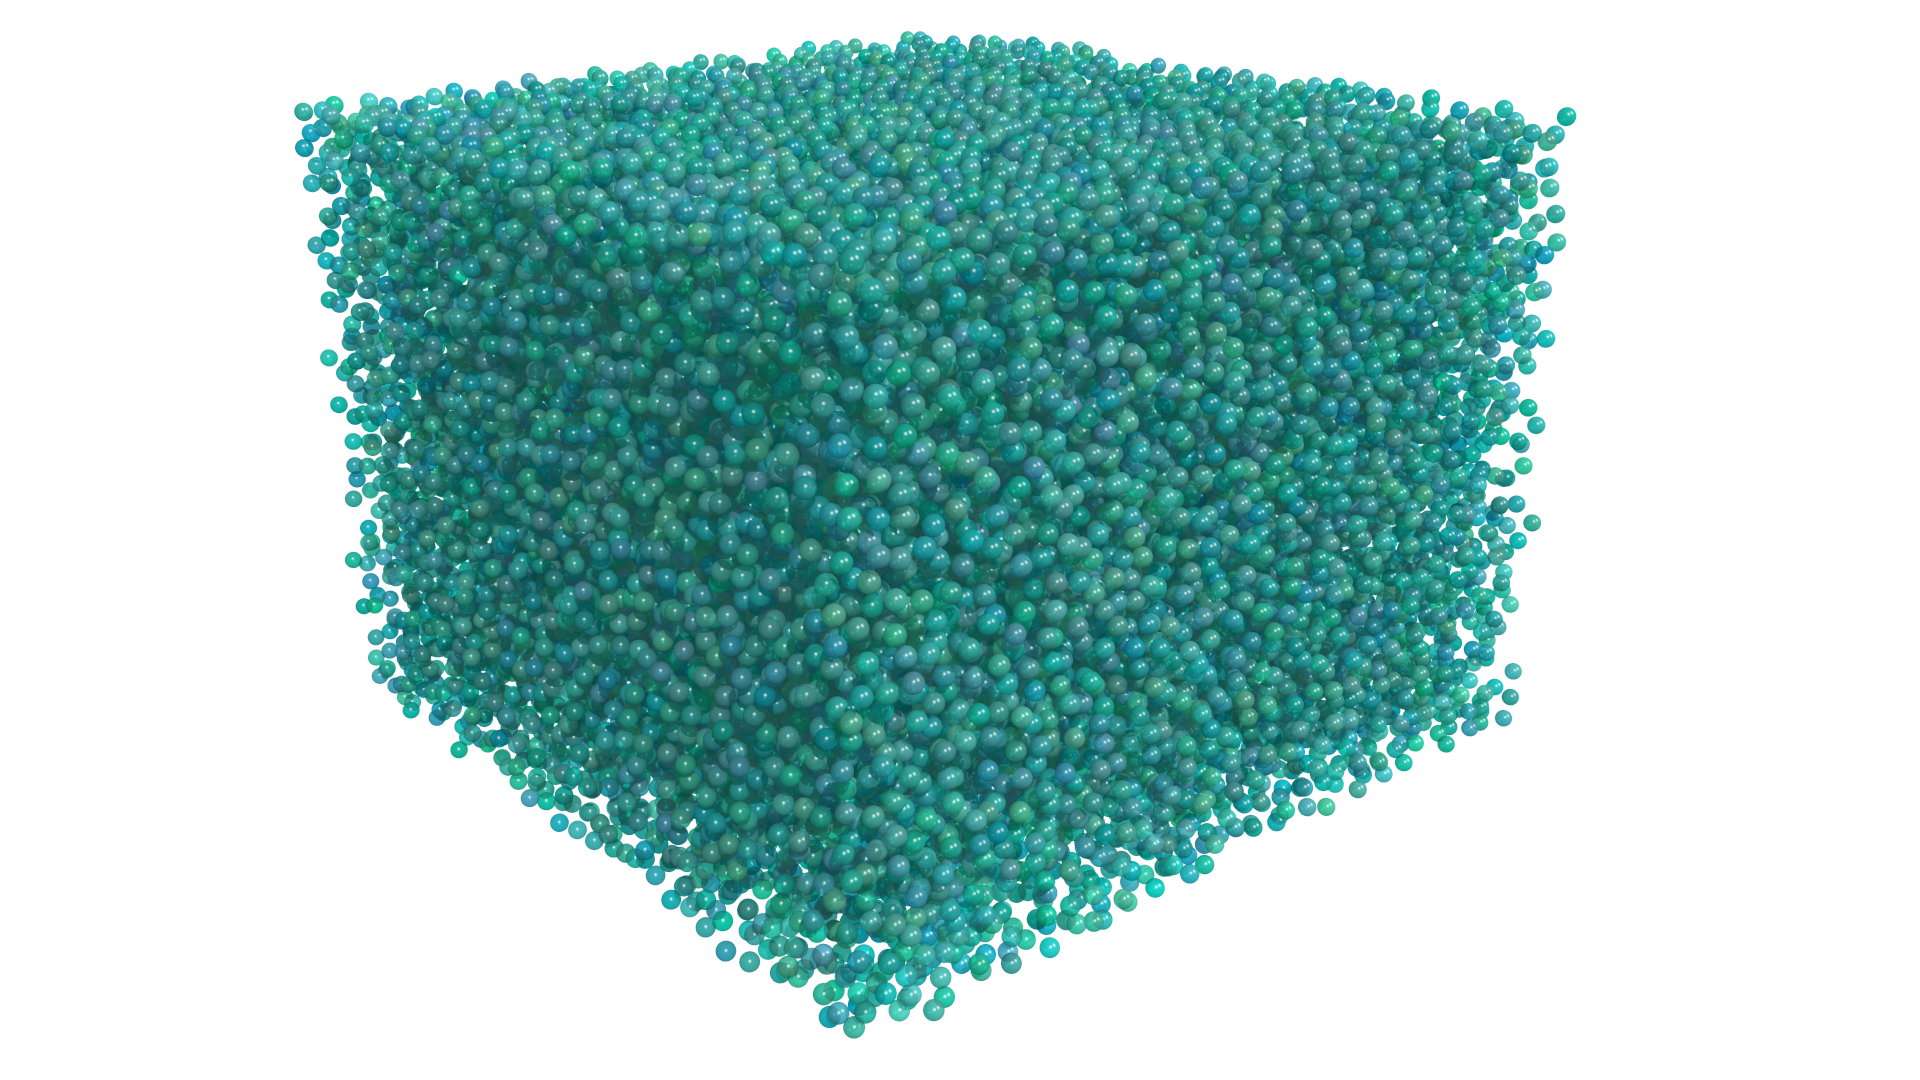
\includegraphics[width=.5\linewidth]{temp_wo_walls}}
\end{frame}
\begin{frame}{The system}
  \frame{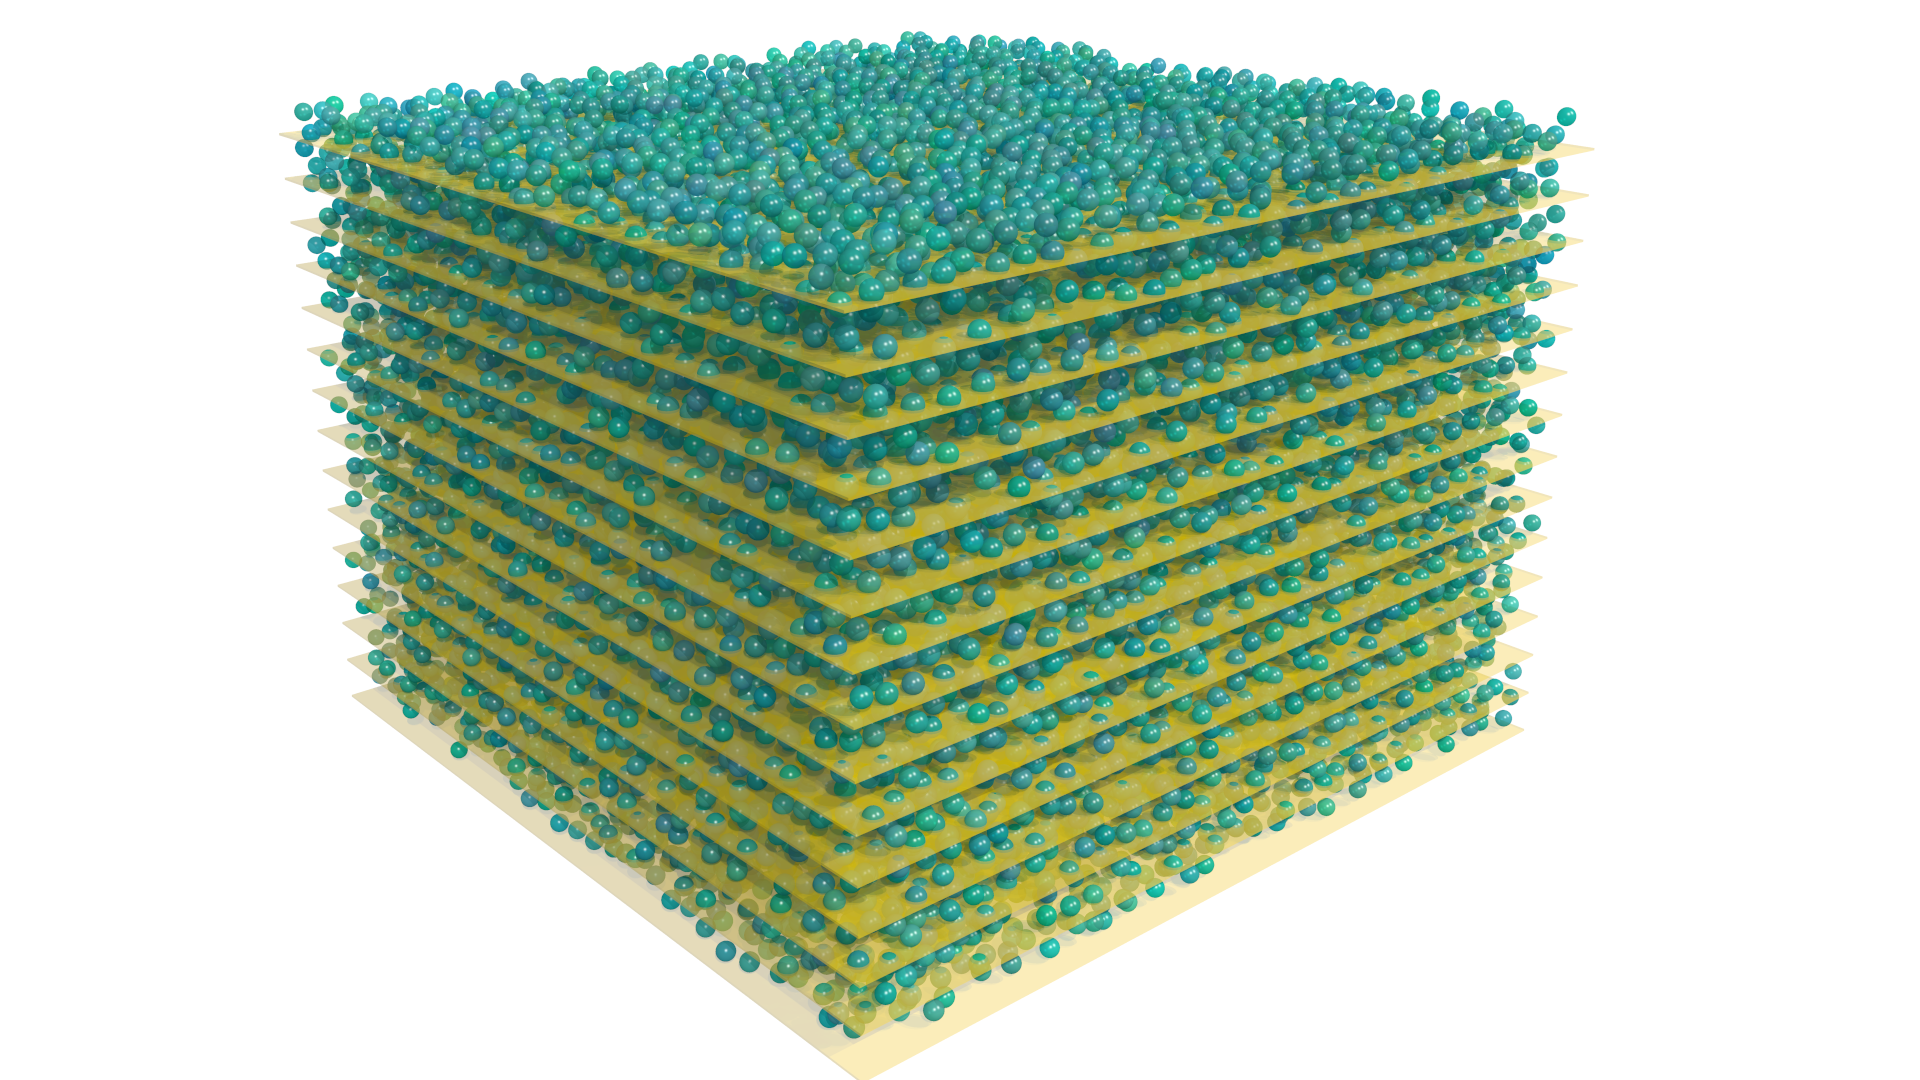
\includegraphics[width=.5\linewidth]{temp_wo_walls_w_layers2}}
\end{frame}

\section{NonMarkovian behaviour}
\begin{frame}{Nonmarkovian}
Texto
\end{frame}
\begin{frame}{The system}
  \frame{\includegraphics[width=.5\linewidth]{PRL3_gold2_wo_diffuse}}
\end{frame}

\section{Conclusions and future directions}
\begin{frame}{Conclusions}
  \begin{itemize}
    \item
    \item
  \end{itemize}
\end{frame}
\begin{frame}{Future directions}
  \begin{itemize}
    \item
    \item
  \end{itemize}
\end{frame}

\section{References and publications}
\begin{frame}{References}
\bibliographystyle{unsrt}
\bibliography{bibTex/thesis-library}
\end{frame}
\begin{frame}{Publications}
  \begin{itemize}
    \item
    \item
    \end{itemize}
\end{frame}

\begin{frame}{}
  \centering
  Muchas gracias
  \includegraphics[width=2.5cm]{logo}
\end{frame}

\end{document}
